\subsection{Heat equation on an unbounded domain}
When the spatial variable ranges over $ \mathbb{R}$, we'll use Fourier transform instead of Fourier series in order to find solution. Therefore, let us first recall its definition. If $f : \mathbb{R} \to \mathbb{C}$ the Fourier transform is given as 
\begin{align*} 
	\mathcal{F}\left[f\right]\left(a\right) = \hat{f}\left(a\right) = \frac{1}{\sqrt{2\pi}} \int_{-\infty}^{\infty}e^{-iax}f\left(x\right)dx
\end{align*}
Where well defined if $\int_{-\infty}^{\infty}\left|f\left(x\right)\right|dx < \infty$. Before solving PDEs, we first need to recall some important properties about Fourier transform.
\begin{align*} 
	\mathcal{F}\left[f'\right]\left(a\right) = ia \mathcal{F}\left[f\right]\left(a\right)\\
	\mathcal{F}\left[f\right]\left(a\right)\mathcal{F}\left[g\right]\left(a\right) = \frac{1}{\sqrt{2\pi}}\mathcal{F}\left[f \ast g\right]\left(a\right)
\end{align*}
Given this, let us define the heat equation 
\begin{parag}{Heat equation}
	\begin{definition}{Heat equation}
    \begin{align*} 
		\begin{cases}
			\frac{\partial u}{\partial t}  - \frac{\partial^2 u}{\partial x^2} = f \mathspace \forall t > 0, x \in \mathbb{R}\\
			u \left(x, 0\right) = u_0\left(x\right)
		\end{cases} 
	\end{align*}
	\end{definition}
	Assuming $\int_{-\infty}^{\infty} \left|u_0\left(x\right)\right|dx < \infty$ and $\int_{-\infty}^{\infty}\left|f\left(x, t\right)\right|dx < \infty$ for every $t > 0$. Therefore, we can take the Fourier transform in $x$ for each part of the equations which gives 
	\begin{align*} 
		\hat{u}\left(a, t\right) = \frac{1}{\sqrt{2\pi}}\int_{-\infty}^{\infty}e^{-iax}u\left(x, t\right)dx\\
		\hat{u}_0\left(x\right) = \frac{1}{\sqrt{2\pi}}\int_{-\infty}^{\infty}e^{-iax}u_0\left(x\right)dx\\
		\hat{f}\left(a, t\right)= \frac{1}{\sqrt{2\pi}}\int_{-\infty}^{\infty}e^{-iax}f\left(x, t\right)dx
	\end{align*}
	Then, we can therefore apply the Fourier transform to the PDE 
	\begin{align*} 
		\frac{\partial u}{\partial t}  - \frac{\partial^2 u}{\partial x^2} = f \implies \mathcal{F}\left[\frac{\partial u}{\partial t}  - \frac{\partial^2 u}{\partial x^2}\right]\left(a, t\right)= \hat{f}\left(a, t\right)
	\end{align*}
	This implies for us the following 
	\begin{align*} 
		\begin{cases}
			\frac{\partial \hat{u}}{\partial t} \left(a, t\right) + a^2 \hat{u}\left(a, t\right) = \hat{f}\left(a, t\right)\\
			\hat{u}\left(a, 0\right) =  \hat{u}_0
		\end{cases} 
	\end{align*}
	Here for each frequency $a \in \mathbb{R}$, this is an \important{ODE in time}. We can therefore find the solution by using the Laplace transform in $t$ 
	\begin{align*} 
		\hat{u}\left(a, t\right) = e^{-a^2t}\hat{u}_0\left(a\right) + \int_{0}^{t}e^{-a^2\left(t-s\right)}\hat{f}\left(a, s\right)ds
	\end{align*}
	To get $u\left(x, t\right)$ we therefore need to apply the inverse Fourier transform. To do so let us first recall some of those 
	\begin{align*} 
		\mathcal{F}\left[e^{-\frac{x^2}{2}}\right]\left(a\right) = e^{-\frac{a^2}{2}}\\
		\mathcal{F}\left[f\left(\lambda x\right)\right]\left(a\right) = \frac{1}{\left|\lambda\right|} \mathcal{F}\left[f\right]\left(\frac{a}{\lambda}\right)
	\end{align*}
	Therefore we obtain 
	\begin{align*} 
		e^{-a^2t}&= e^{- \frac{\left(\sqrt{2t}a\right)^2}{2}}\\
				&= \frac{1}{\sqrt{2t}}\mathcal{F}\left[e^{-\frac{\left(\frac{x}{\sqrt{2t}}\right)^2}{2}}\right]\left(a\right)\\
				&= \mathcal{F}\left[\frac{1}{\sqrt{2t}}e^{-\frac{x^2}{4t}}\right]\left(a\right)
	\end{align*}
	Which therefore implies 
	\begin{align*} 
		\hat{u}\left(a, t\right) = \mathcal{F}\left[\frac{1}{\sqrt{2t}}e^{-\frac{x^2}{4t}}\right]\left(a\right)\mathcal{F}\left[u_0\right]\left(a\right) + \int_0^{t}\mathcal{F}\left[\frac{1}{\sqrt{2\left(t-s\right)}}e^{-\frac{x^2}{4\left(t-s\right)}}\right]\left(a\right)\mathcal{F}\left[f\left(x, s\right)\right]\left(a\right)ds
	\end{align*}
	Using the property about convolutions and inverting we get 
	\begin{align*} 
		u\left(x, t\right) = \frac{1}{\sqrt{2\pi}}\int_{-\infty}^{\infty}\frac{1}{\sqrt{2t}}e^{-\frac{\left(x -y\right)^2}{4t}} u_0\left(y\right)dy + \frac{1}{\sqrt{2\pi}}\int_0^{t}\int_{-\infty}^{\infty}\frac{1}{\sqrt{2\left(t-s\right)}}e^{-\frac{\left(x-y\right)^2}{4\left(t-s\right)}} f\left(y, s\right)dyds
	\end{align*}
\end{parag}



\subsection{Wave equation on an unbounded interval}
\begin{definition}{Wave equation on an unbounded interval}
\begin{align*} 
	\begin{cases}
		\frac{\partial^2u}{\partial t^2} - \frac{\partial^2u}{\partial x^2} = f \mathspace \mathspace \forall t > 0, x \in \mathbb{R}\\
		u\left(x, 0\right) = u_0\left(x\right)\\
		\frac{\partial u}{\partial t} \left(x, 0\right)= u_1\left(x\right)
	\end{cases} 
\end{align*}
\end{definition}
Here we will use the same strategy as for the heat equation: we first apply the Fourier transform in $x$ to the PDE. We will then get an ODE (in $t$) for the Fourier transform which we will be able to solve. Finally, we will then invert it. Using this trick 
\begin{align*} 
	\frac{\partial^2 u}{\partial t^2}  - \frac{\partial^2 u}{\partial x^2}  = f \implies \mathcal{F}\left[\frac{\partial^2 u}{\partial t^2}  - \frac{\partial^2 u}{\partial x^2}\right] = \mathcal{F}\left[f\right]
\end{align*}
If we developed this we get 
\begin{align*} 
	\begin{cases}
		\frac{\partial^2 \hat{u}}{\partial t^2} \left(a, t\right) + a^2 \hat{u}\left(a, t\right) = \hat{f}\left(a, t\right) \mathspace \mathspace \forall t > 0, a \in \mathbb{R}\\
		\hat{u}\left(a, 0\right) = \hat{u}_0\left(a\right)\\
		\frac{\partial \hat{u}}{\partial t} \left(a, 0\right)= \hat{u}_1\left(a\right)
	\end{cases} 
\end{align*}
Again using the Laplace transform 
\begin{align*} 
	\hat{u}\left(a, t\right) = \cos\left(at\right)\hat{u}_0\left(a\right) + \frac{1}{a}\sin\left(at\right)\hat{u}_1\left(a\right) + \int_0^{t}\frac{1}{a}\sin\left(a\left(t-s\right)\right)\hat{f}\left(a, s\right)ds
\end{align*}
Now our goal is to invert the Fourier transform. This is trickier than previously, can the term $\cos\left(at\right)\hat{u}_0\left(a\right)$ be written as a Fourier transform of a single function? To do so we will need to recall this property 
\begin{align*} 
	\mathcal{F}\left[h\left(x + c\right)\right]\left(a\right) = e^{iac}\mathcal{F}\left[h\left(x\right)\right]\left(a\right)
\end{align*}
Using this fact and by developing our $\cos\left(at\right)$, we get 
\begin{align*} 
	\hat{u}_0\left(a\right)\cos\left(at\right) = \hat{u}_0\left(a\right)\frac{e^{ait} + e^{-iat}}{2} = \frac{1}{2}\mathcal{F}\left[u_0\left(x + t\right) + u_0\left(x -t\right)\right]\left(a\right)
\end{align*}
However for the $\frac{1}{a}\sin\left(at\right)\hat{u}_1\left(a\right)$ this won't work, we need to find a way to also  '\textit{incorporer}' (j'ai pas le mot anglais) the $\frac{1}{a}$ into the transform. To do so we will use the following function 
\begin{align*} 
	h\left(x\right) = \begin{cases}
		1 \mathspace -1 \leq x \leq 1 \\ 0 \mathspace \text{ otherwise }
	\end{cases}  \implies \hat{h}\left(a\right) = \sqrt{\frac{2}{\pi}}\frac{\sin\left(a\right)}{a}
\end{align*}
Using the rescaling property and the fact $h_t\left(x\right) = h\left(\frac{x}{t}\right)$ where 
\begin{align*} 
	h_t\left(x\right) = \begin{cases}
		1 \mathspace -t \leq x \leq t \\ 0 \mathspace \text{ otherwise}
	\end{cases} 
\end{align*}
We can the compute that
\begin{align*} 
	\hat{h}_t\left(a\right) = \sqrt{\frac{2}{\pi}}\frac{\sin\left(at\right)}{a}
\end{align*}
And then reinserting this into our equation 
\begin{align*} 
	\hat{u}_1\left(a\right)\frac{\sin\left(at\right)}{a} &= \mathcal{F}\left[u_1\right]\left(a\right)\sqrt{\frac{\pi}{2}}\mathcal{F}\left[h_t\right]\left(a\right)\\
	&= \frac{1}{2}\mathcal{F}\left[u_1 \ast h_t\right]\left(a\right)
\end{align*}

And we can also see that the convolution here will be simplified a lot by the $h_t$ function right?
\begin{align*} 
	u_1 \ast h_t \left(x\right) = \int_{-\infty}^{\infty}h_t\left(x - y\right)u_1\left(y\right)dy = \int_{x-t}^{x + t}u_1\left(y\right)dy
\end{align*}
We can then take the overall invertation of $\hat{u}$ which gives us 
\begin{align*} 
	u\left(x, t\right) = \frac{1}{2}\left[u_0\left(x + t\right) + u_0\left(x -t\right)\right] + \frac{1}{2}\int_{x-t}^{x + t}u_1\left(y\right)dy + \frac{1}{2}\int_0^{t}\int_{x-t}^{x + t}f\left(y, s\right)dyds
\end{align*}



\subsection{Shrödinger equation on an unbounded interval}

\begin{definition}{Shrödinger equation}
	Suppose $u : \mathbb{R} \times \left(0, x_0\right) \to \mathbb{C}$ solves 
	\begin{align*} 
		i \frac{\partial u}{\partial t} \left(x, t\right) + \frac{\partial^2 u}{\partial x^2} \left(x, t\right) - v\left(x, t\right)u\left(x, t\right) = 0 \mathspace \mathspace \forall t > 0, x \in \mathbb{R}
	\end{align*}
	The Shrödinger equation write the potential
\end{definition}
\begin{parag}{properties}
    \begin{itemize}
        \item The potential is always assumed to be real values
        \item Hence, $u$ is necessarily complex-valued in view of the imaginary unit of the equation
    \end{itemize}
	\begin{subparag}{Physical interpretation}
	    The Shrödinger equation describes the evolution of a quantum particle moving under the influence of a classical potential.
	\end{subparag}
\end{parag}
\begin{parag}{Facts}
    \begin{itemize}
		\item The energy is conserved (probabilistic interpretation):
	\begin{align*} 
		\int_{-\infty}^{\infty} \left|u\left(x, t\right)\right|^2 dx \mathspace \text{ constant in }t
	\end{align*}
	\item \textbf{Uniqueness} two solutions with the same initial conditions necessarily coincide
	\item \textbf{Existence} Assuming for simplicity $v= 0$, arguing by Fourier transform as for the heat equation we find 
		\begin{align*} 
			u\left(x, t\right) = \frac{1}{\sqrt{2\pi it}}\int_{-\infty}^{\infty}e^{-\frac{\left(x-y\right)^2}{4it}}u_0\left(y\right)dy - i \int_0^{t}\int_{-\infty}^{\infty}\frac{1}{\sqrt{4\pi i \left(t-s\right)}}e^{-\frac{\left(x-y\right)^2}{4i\left(t-s\right)}}f\left(y, s\right)ds
		\end{align*}
    \end{itemize}
	\begin{subparag}{Note}
	    We can compare this to the heat equation to convince ourself that this is indeed a solution.
	\end{subparag}
\end{parag}


\begin{parag}{Example}
    Assume $f= 0$, $u_0\left(x\right)= e^{-\frac{x^2}{2}}$. Then $\hat{u}_0\left(a\right)= e^{-\frac{a^2}{2}}$ so 
	\begin{align*} 
		\hat{u}\left(a, t\right) = e^{-ia^2b}\hat{u}_0\left(a\right) = e^{-ia^2t}e^{-\frac{a^2}{2}} = e^{-\left(it + \frac{1}{2}\right)a^2}
	\end{align*}
	Which implies
	\begin{align*} 
		u\left(x, t\right) = \frac{1}{\sqrt{2\pi}}\int_{-\infty}^{\infty}e^{iax}e^{-\left(it + \frac{1}{2}\right)a^2}da
	\end{align*}
	This integral can be computed explicitly using complex integration. The idea is to reduce this task to a known integral (here Gaussian integral). Setting 
	\begin{align*} 
		z = \left(a - \frac{ix}{2it - 1}\right)\sqrt{2it - 1}
	\end{align*}
	So that 
	\begin{align*} 
		e^{ixa - \left(it + \frac{1}{2}\right)a^2} = e^{-\frac{x^2}{4it + 2}}e^{-\frac{z^2}{2}}
	\end{align*}
	\begin{subparag}{Remark}
	Note when $a$ goes from $-\infty$ to $\infty$, $z = z\left(a\right)$ parametries a straight line $\gamma$ through $\mathbb{C}$.
	\end{subparag}
	\begin{center}
	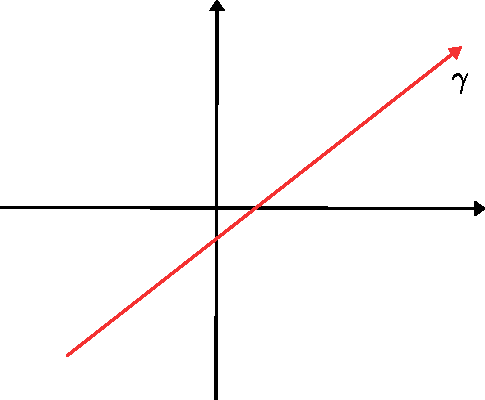
\includegraphics[width=0.4\textwidth]{figure/2026-05-29.pdf}
	\end{center}
	Let us now  compute $u$
	\begin{align*} 
		u\left(x, t\right)&= \frac{1}{\sqrt{2\pi}}\int_{-\infty}^{\infty}e^{ixa - \left(it + \frac{1}{2}\right)a^2}da \\
						  &= \frac{1}{\sqrt{2\pi}}\int_{\gamma}e^{-\frac{x^2}{\left(4it + 2\right)}}e^{-\frac{x^2}{2}}\frac{dz}{\sqrt{2it + 1}}\\
						  &= \frac{1}{\sqrt{2\pi}}\frac{e^{-\frac{x^2}{\left(4it + 2\right)}}}{\sqrt{2it + 1}} \int_{\gamma}e^{-\frac{z^2}{2}}dz
	\end{align*}
	Using Cauchy's theorem, we can move the integration curve from $\gamma$ to $ \mathbb{R}$. To do so will define the new curve with $\sigma_1, \sigma_2$:
	\begin{center}
	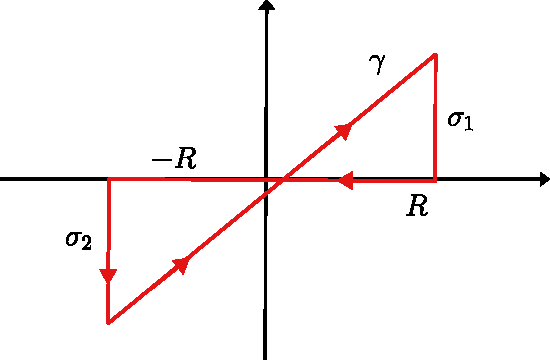
\includegraphics[width=0.6\textwidth]{figure/2026-05-29_1.pdf}
	\end{center}
	But before being sure that this works well we first need to note that 
	\begin{align*} 
		\int_{\sigma_1}e^{-\frac{z^2}{2}}dz, \int_{\sigma_2}e^{-\frac{z^2}{2}}dz \to 0 \text{ as } R\to \infty
	\end{align*}
	While 
	\begin{align*} 
		\int_{-R}^{R}e^{-\frac{z^2}{2}}dz \to \int_{-\infty}^{\infty}e^{-\frac{z^2}{2}}dz = \sqrt{2\pi}
	\end{align*}
	In summary, we have 
	\begin{align*} 
		u\left(x, t\right) = \frac{e^{-\frac{x^2}{\left(4it + 2\right)}}}{\sqrt{2it + 1}}
	\end{align*}
\end{parag}









